% ---------------------------------------------------------------------------
% The result of comparing the sampled per-site entropy of the zero_polymer
% chains with the natural per-site entropy of influenza A HA, now that the
% cross-subtype entropy files exist. Method and definitions:
% ha_natural_methods.tex; commands: softmax/monte_carlo/ha_natural_runbook.md.
%
% Figure: regenerate with make_ha_entropy_result_fig.py (run from softmax/monte_carlo).
% Build:  cd softmax/docs && pdflatex ha_entropy_result.tex && pdflatex ha_entropy_result.tex
% ---------------------------------------------------------------------------
\documentclass[11pt,a4paper]{article}

\usepackage[T1]{fontenc}
\usepackage[utf8]{inputenc}
\usepackage[margin=2.5cm]{geometry}
\usepackage{amsmath,amssymb}
\usepackage{booktabs}
\usepackage{graphicx}
\usepackage[hidelinks]{hyperref}
\sloppy

\newcommand{\file}[1]{\texttt{#1}}
\newcommand{\Neff}{N_{\mathrm{eff}}}

\title{Does the sampler conserve what the protein conserves?\\
       \large The zero\_polymer chains against cross-subtype HA entropy}
\author{}
\date{3 November 2026}

\begin{document}
\maketitle

\begin{abstract}
\noindent
The sampler's conserved sites \emph{are} significantly enriched among the sites
influenza A hemagglutinin really conserves: the 53 K-sites of the T12 chain
overlap the naturally conserved sites 3 times more often than chance, at
$p \approx 10^{-7}$. But they are in the \emph{wrong part} of the protein. The
prediction written down before the data existed was that the sampler should lock
the HA2 stalk; instead the K-sites are depleted in HA2 by a factor 3.4 and
concentrated in the HA1 head, specifically around the receptor-binding site,
where they are enriched 3.3-fold. The site-by-site rank correlations stay small
throughout (0.06 to 0.10 at T12). The cross-subtype files are what made any of
this measurable: on the old human-H3N2 file the same test has no power at all
($p = 0.27$), because 81\% of that protein looks conserved.
\end{abstract}

\section{What was run}

Four natural entropy files, all built with \file{ha\_site\_entropy.py} from HA
sequences fetched from NCBI Protein (16 subtypes, H1--H16; the counts are in
Table~\ref{tab:data}):

\begin{center}
\begin{tabular}{@{}llrr@{}}
\toprule
file & subtypes & $\Neff$ & NaN sites \\
\midrule
\file{ha\_group2\_entropy\_566.csv} & group 2 (6), $\theta = 0.8$  &  8.1 & 12 \\
\file{ha\_group2\_w95\_566.csv}     & group 2 (6), $\theta = 0.95$ & 81.8 &  9 \\
\file{ha\_allA\_entropy\_566.csv}   & all A (16), $\theta = 0.8$   & 15.7 & 16 \\
\file{ha\_allA\_w95\_566.csv}       & all A (16), $\theta = 0.95$  & 234.3 & 16 \\
\midrule
\file{FASTA/H3N2/site\_entropy\_566.csv} & human H3N2 only & (unweighted) & 0 \\
\bottomrule
\end{tabular}
\end{center}

\noindent
against the sampled per-site entropy already in
\file{nsites\_study/structure/site\_entropy\_by\_T.csv}: T5 and T12 (one chain
each), T32 (two chains pooled) and T100 (four chains).

\section{The data behind the natural files}
\label{sec:data}

\begin{table}[h]
\centering
\caption{Per-subtype composition of the all-A files, from
\file{ha\_allA\_w95\_566.summary.tsv}. ``Unique'' counts distinct sequences after
filtering; \file{--max-unique} caps each subtype at 3\,000, which bound H1, H3
and H5 only. Identity is the median over that subtype to the \file{zero\_polymer}
reference, after alignment.}
\label{tab:data}
\small
\begin{tabular}{@{}lrrrrr@{}}
\toprule
subtype & raw & unique & kept & $\Neff$ at 0.95 & identity to ref \\
\midrule
H1  & 28\,717 & 13\,541 & 3\,000 & 66.1 & 0.417 \\
H3  & 26\,377 & 11\,617 & 3\,000 & 42.7 & 0.959 \\
H5  &  6\,718 &  4\,741 & 3\,000 & 23.5 & 0.399 \\
H9  &  3\,678 &  2\,707 & 2\,707 & 22.1 & 0.392 \\
H7  &  3\,201 &  1\,712 & 1\,712 & 19.3 & 0.473 \\
H6  &  1\,821 &  1\,408 & 1\,408 & 16.3 & 0.403 \\
H4  &  2\,012 &  1\,157 & 1\,157 &  6.2 & 0.650 \\
H10 &  1\,170 &    622  &   622  &  5.8 & 0.482 \\
H11 &     665 &    590  &   590  &  6.3 & 0.405 \\
H2  &     629 &    483  &   483  &  5.1 & 0.389 \\
H13 &     509 &    258  &   258  &  8.4 & 0.380 \\
H12 &     223 &    201  &   201  &  2.1 & 0.403 \\
H16 &     262 &    141  &   141  &  6.0 & 0.376 \\
H8  &     161 &    151  &   151  &  1.1 & 0.403 \\
H14 &      30 &     20  &    20  &  1.3 & 0.643 \\
H15 &      22 &     11  &    11  &  2.0 & 0.475 \\
\bottomrule
\end{tabular}
\end{table}

Two things in this table matter for reading the result.

\paragraph{The identities confirm the mapping worked.}
H3 comes out at 0.959 to the reference, as it should, since the reference is an
H3. H4 at 0.650 and H14 at 0.643 are the next closest, which is exactly the
group~2 structure expected from the phylogeny, and every group~1 subtype sits
near 0.40. Nothing is mis-mapped.

\paragraph{At $\theta = 0.8$ the weighting over-corrects.}
The $\Neff$ column at $\theta = 0.8$ (not shown above; in the
\file{\_entropy\_566.summary.tsv} files) is 1.0 for most subtypes, as expected,
but 0.0 for H15, 0.4 for H16 and 0.7 for H13. Those are not bugs: sister
subtypes are more than 80\% identical to each other, so H15 (11 unique
sequences) is absorbed into the H7 cluster (1\,712 sequences) and ends up with
essentially zero total weight, and H13/H16 absorb each other. So at 0.8 the
entropy is not ``one vote per subtype'' as the runbook suggests, it is one vote
per \emph{cluster of sister subtypes}, with small subtypes next to large ones
silently dropped. \textbf{Prefer the $\theta = 0.95$ files}; this was not
something I anticipated when writing the method, and it is the one correction to
make to \file{ha\_natural\_methods.tex}.

\section{Result 1: the natural files behave as predicted}

The prediction was HA2 conserved, HA1 head variable. On the natural side it
holds, and more cleanly in the cross-subtype files than in H3N2 (median per-site
entropy, bits; signal peptide 0--15, HA1 16--344, HA2 345--565, the HA2 boundary
located from the fusion peptide motif \texttt{GIFGAIAGF} at index 345):

\begin{center}
\begin{tabular}{@{}lrrr@{}}
\toprule
file & signal & HA1 & HA2 \\
\midrule
group 2, $\theta = 0.8$  & 1.993 & 1.478 & 0.812 \\
group 2, $\theta = 0.95$ & 2.092 & 1.276 & \textbf{0.454} \\
all A, $\theta = 0.8$    & 2.704 & 1.809 & 0.991 \\
all A, $\theta = 0.95$   & 2.616 & 1.709 & 1.060 \\
human H3N2               & 0.049 & 0.015 & 0.007 \\
\bottomrule
\end{tabular}
\end{center}

\noindent
HA2 is about a third of HA1's entropy in the group~2 file at $\theta = 0.95$,
and the signal peptide is the most variable region of all, which is correct: it
is cleaved off and only its hydrophobicity is under selection. The pipeline is
measuring what it was built to measure.

Look at the H3N2 row, though. Its numbers are 20 to 100 times smaller, because
within one lineage almost nothing varies at all. That is the quantitative
version of the argument for doing this work, and Section~\ref{sec:power} is
where it bites.

\section{Result 2: the sampler conserves real sites, in the wrong place}

The K-sites are the sites with sampled entropy below 0.05 at the cold labels.
\textbf{Only T12 is usable.} The T5 chain accepted 179 mutations over 566 sites,
0.32 per site, so its 518--520 ``conserved'' sites are overwhelmingly sites the
chain never touched, not sites it refused to change. T12 accepted 26\,666
mutations over 1\,001 kept checkpoints, 47 per site, so its 53 K-sites mean
something. Everything below is T12.

\paragraph{The overlap is real.}
Against the group~2 $\theta = 0.95$ file, 23 of the 53 K-sites are among the 83
sites with natural entropy below 0.1 bits, where chance would give 7.9:
$p = 9.9\times10^{-8}$. The same test on the other files gives
$p = 2.9\times10^{-6}$ (group 2, 0.8), $6.2\times10^{-6}$ (all A, 0.95) and
$6.7\times10^{-5}$ (all A, 0.8). The median natural entropy at the K-sites is
0.338 bits against 1.076 at the remaining sites. So the sites the sampler
refuses to change are, as a set, genuinely unusually conserved in nature. This
is the positive result, and it is not marginal.

\paragraph{But they are in the head, not the stalk.}
\begin{center}
\begin{tabular}{@{}lrrrr@{}}
\toprule
region & sites & K-sites & expected if uniform & enrichment \\
\midrule
signal (0--15)   &  16 &  1 &  1.5 & 0.67 \\
HA1 (16--344)    & 329 & \textbf{46} & 30.8 & \textbf{1.49} \\
HA2 (345--565)   & 221 & \textbf{6}  & 20.7 & \textbf{0.29} \\
\bottomrule
\end{tabular}
\end{center}

\noindent
This is the opposite of the prediction. HA2, the region the natural alignment
says is the most constrained part of the molecule, is where the sampler is
\emph{least} likely to hold a site fixed. Of the 6 K-sites that are in HA2,
only 1 is naturally conserved. Within HA2 alone the rank correlation between
sampled and natural entropy is 0.074, i.e. nothing.

The one pleasing detail is that index 345, the very first residue of HA2 and so
the first residue of the fusion peptide, \emph{is} a K-site. The sampler found
the single most famous constrained residue in the molecule and then ignored the
rest of the stalk.

\paragraph{What the HA1 K-sites are.}
They are not scattered through the head. Sixteen of the 53 fall inside the
classic receptor-binding neighbourhoods (H3 numbering 130--140, 150--160,
183--200, 219--229), which are only 52 of 566 sites, so chance would give 4.9:
a 3.3-fold enrichment. In H3 numbering the K-sites include an almost unbroken
run 190--200 (190, 191, 192, 193, 194, 195, 196, 197, 198, 199, 200) and a
second cluster 239--263. The 190-helix is a core element of the receptor-binding
site.

Three checks that this is not noise:
\begin{itemize}
  \item \textbf{Spatial clustering.} The 53 K-sites form 36 contiguous runs; 53
    sites placed at random form $48.1 \pm 2.0$ runs, so the clustering is far
    beyond chance ($P \le 36$ is below $10^{-4}$ over 20\,000 draws). The
    sampler is freezing structural neighbourhoods, not isolated positions.
  \item \textbf{Temperature consistency.} The T32 chains, a different
    temperature and two pooled chains, give 13 K-sites, and 12 of those 13 are
    also K-sites at T12. The cold-chain conserved set is reproducible and not an
    artifact of one trajectory.
  \item \textbf{Mutational opportunity.} At T100 no site at all has entropy
    below 0.05, so the proposal mechanism does reach every site; a frozen site
    at T12 is a rejection, not an absence of attempts.
\end{itemize}

\paragraph{The rank correlations are small everywhere.}
\begin{center}
\begin{tabular}{@{}lrrrr@{}}
\toprule
natural file & T5 & T12 & T32 & T100 \\
\midrule
group 2, $\theta = 0.8$  & 0.124 & 0.063 & 0.014 & 0.038 \\
group 2, $\theta = 0.95$ & 0.120 & 0.077 & 0.035 & 0.050 \\
all A, $\theta = 0.8$    & 0.122 & 0.083 & 0.029 & 0.025 \\
all A, $\theta = 0.95$   & 0.145 & 0.104 & 0.025 & 0.020 \\
human H3N2               & 0.131 & 0.086 & $-0.040$ & 0.023 \\
\bottomrule
\end{tabular}
\end{center}

\noindent
Do not read the T5 column: as above, that entropy is mostly an artifact of too
few accepted mutations, and its apparently ``best'' correlation is the least
meaningful number in the table. At T12 the honest figure is 0.06--0.10. The
correlation falls with temperature, which is at least the right direction: the
hotter chains look less like the natural protein. But a site-by-site
correlation of 0.08 is weak, and the result has to rest on the K-site overlap,
which is a statement about the extremes of the distribution, not about the
distribution as a whole.

\section{Result 3: this is why the cross-subtype files were needed}
\label{sec:power}

On the human-H3N2 file, 457 of 566 sites have entropy below 0.1 bits, i.e.\ 81\%
of the protein counts as ``naturally conserved''. The K-site overlap test then
gives 45 observed against 42.8 expected, $p = 0.27$: no signal, because almost
any set of 53 sites would score the same. The cross-subtype files cut
``conserved'' down to 72--131 sites out of 566, and the same 53 K-sites then
come out at $p \approx 10^{-7}$.

So the headline positive finding in this note is one that could not have been
obtained from the old file. The comparison was not merely noisier before, it was
statistically empty.

\section{Figure}

\begin{center}
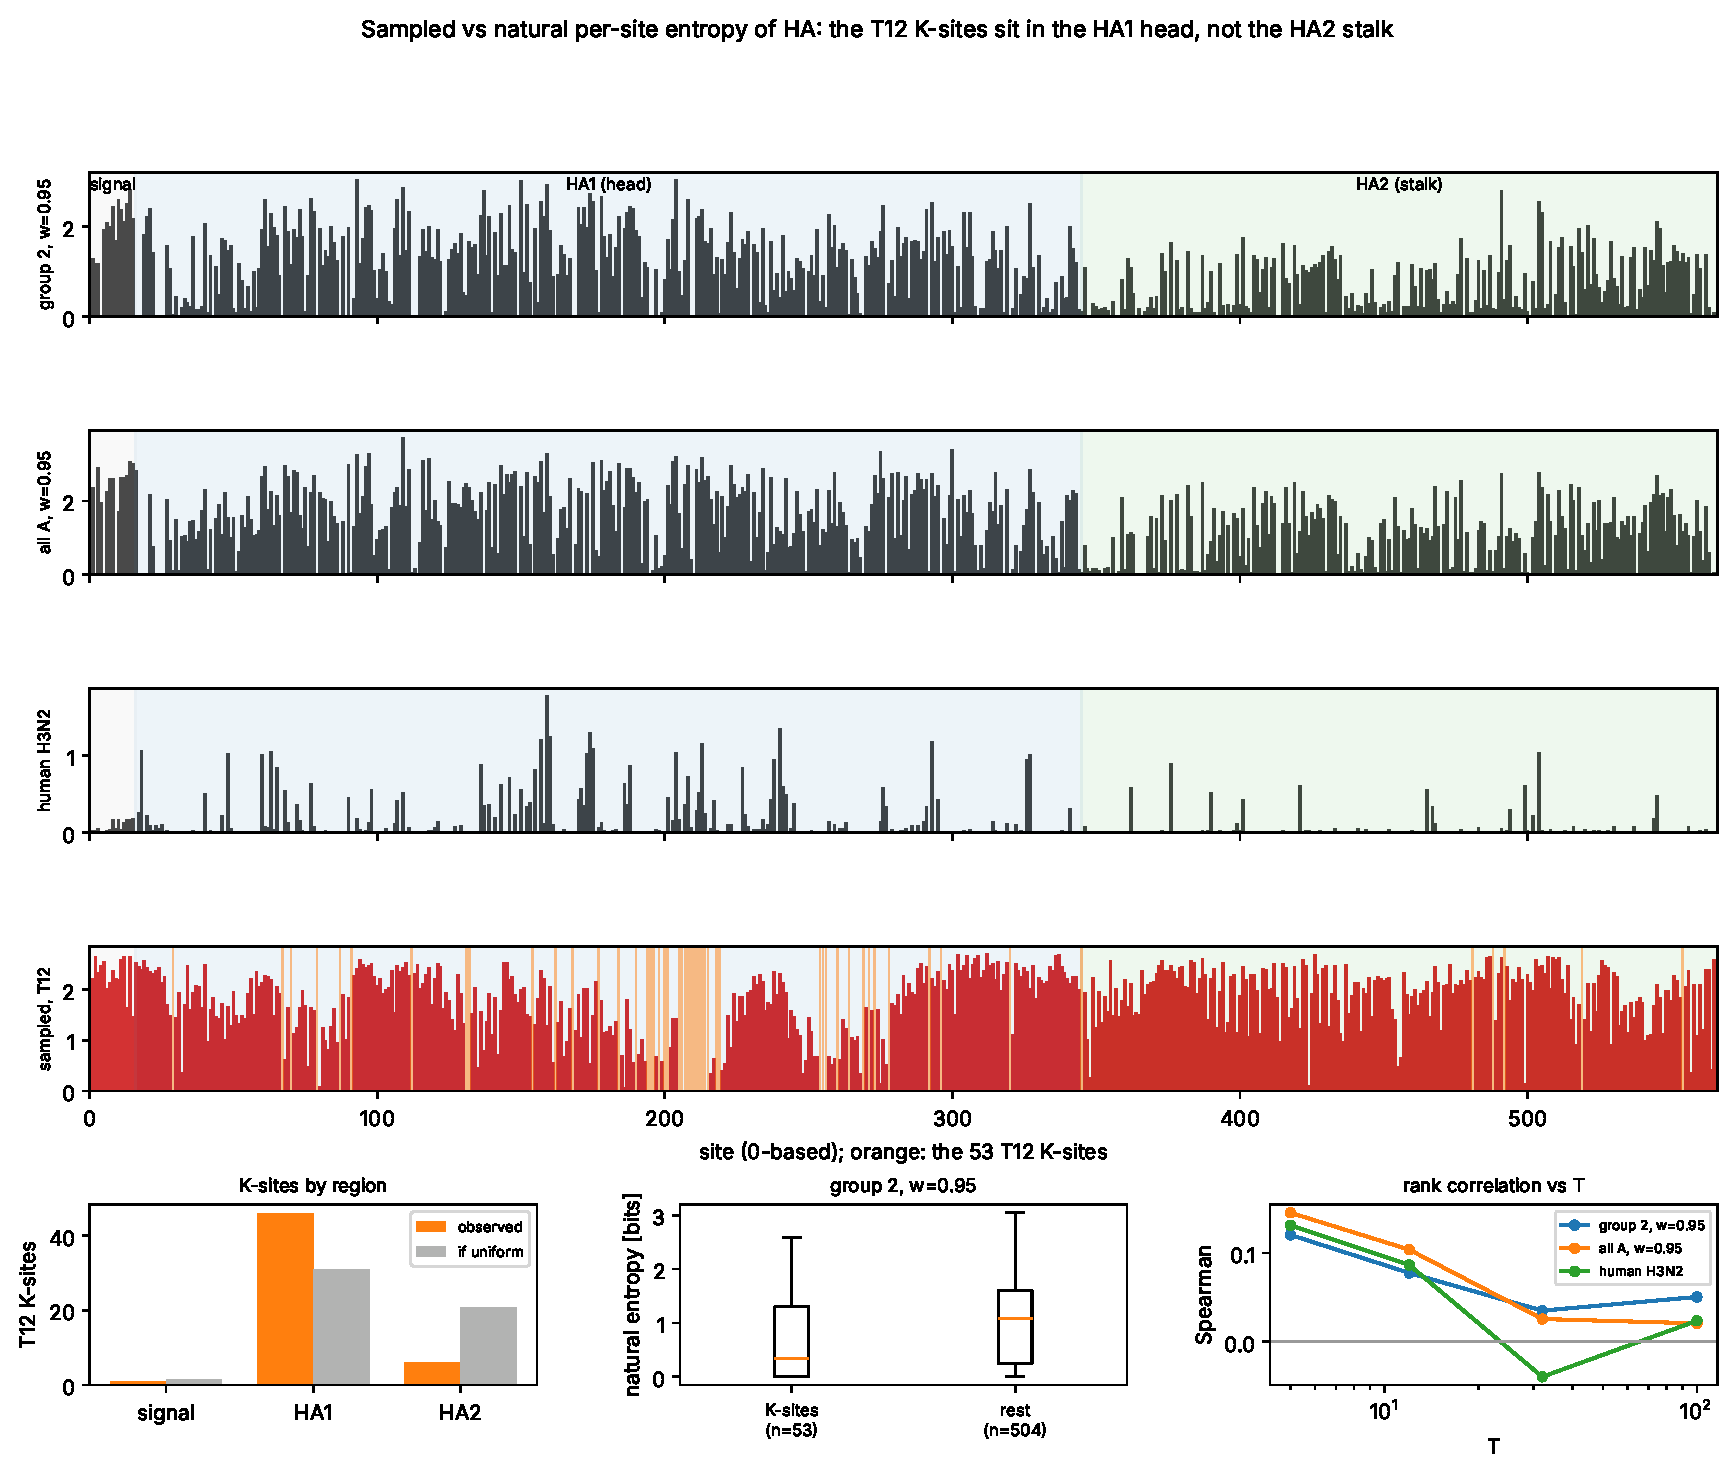
\includegraphics[width=\textwidth]{ha_entropy_result_fig.pdf}
\end{center}

\noindent
Top three panels: natural per-site entropy for group~2 and all-A at
$\theta = 0.95$ and for human H3N2, on the same site axis, with the signal
peptide, HA1 and HA2 spans shaded. Fourth panel: the sampled entropy at T12,
with the 53 K-sites as orange lines; the visible clusters of orange in the
middle of HA1 and their near-absence beyond site 345 are the whole result.
Bottom row: K-sites by region against the uniform expectation, natural entropy
at K-sites against the rest, and the rank correlation against temperature.

\section{How to read this, and what I would do next}

The sampler is not reproducing nothing. It holds a set of sites that is
significantly biased towards genuinely conserved positions, it does so
reproducibly across temperatures, and it freezes contiguous structural
neighbourhoods rather than scattered residues. That is more than a null result.

But it is conserving the \emph{static folded core of the head}, above all the
receptor-binding region, and not the \emph{stalk}. There is a plausible physical
reason, and it is a statement about the energy, not about the sampling: $U$ is a
distance between ESM3 attention maps. Attention maps report on the contacts that
define a rigid, well-packed structure, which the $\beta$-sheet head core and the
receptor-binding site are. The HA2 stalk's natural conservation is of a different
kind: it is conserved because it must be \emph{metastable}, able to undergo the
large pH-triggered rearrangement that drives membrane fusion. Nothing in a
distance between attention maps of the pre-fusion state can see a constraint
whose content is ``this structure has to be able to become a different
structure''. If that reading is right, the mismatch is a property of
$U_{\mathrm{am}}$ as a foldability proxy, and no improvement to the move set
will fix it.

Concretely, in order of how much they would change the story:

\begin{enumerate}
  \item \textbf{Check the energy, not the sampler.} Compute $U$ for the
    reference with single mutations placed (a) at HA2 stalk sites that are
    conserved naturally but free in the sampler, and (b) at the HA1 K-sites.
    If the stalk mutations really do cost little, the mismatch is in $U$ and
    this becomes a finding about the energy function. That is a cheap, decisive
    experiment and I would do it first.
  \item \textbf{Run the comparison on the finished T12 chain.} The numbers here
    use the 1\,001 checkpoints that existed when the entropy file was written.
    The T12 chain has since reached 1M moves; redoing the entropy on the full
    post-burn-in set may move the K-site count.
  \item \textbf{Use the secondary tier.} The 0.05 nat threshold gives 53 sites.
    The paper's ``lower than 1'' tier would give a larger set and a less extreme
    test; if the HA1/HA2 asymmetry survives there too, it is not a threshold
    effect. A sensitivity run at 0.01, 0.05, 0.1 and 0.3 is still outstanding.
  \item \textbf{Fix the $\theta = 0.8$ over-correction} noted in
    Section~\ref{sec:data}, or simply standardise on $\theta = 0.95$ and say
    why.
\end{enumerate}

\paragraph{One caveat on all of it.}
Every number here comes from a single cold chain, T12. The temperature
consistency check with T32 is reassuring but T32 is above the transition. Before
any of this goes in the thesis it wants a second independent cold chain, which
is what the T5 resume was for; at 0.32 accepted mutations per site T5 cannot yet
serve that purpose.

\end{document}
